\documentclass[10pt,twocolumn]{article}
\usepackage[margin=0.68in,top=0.78in,bottom=0.78in,columnsep=0.24in]{geometry}
\usepackage{mathptmx}
\usepackage{amsmath,amssymb,amsthm,amsfonts}
\usepackage{graphicx}
\graphicspath{{figures/}{./}}
\usepackage{booktabs}
\usepackage{array}
\usepackage{enumitem}
\usepackage{xcolor}
\usepackage{titlesec}
\usepackage{caption}
\usepackage{fancyhdr}
\usepackage{lastpage}
\usepackage{microtype}
\usepackage{cite}
\usepackage[colorlinks=true,linkcolor=navy,citecolor=navy,urlcolor=navy]{hyperref}

\definecolor{navy}{RGB}{20,52,92}
\definecolor{slate}{RGB}{71,85,105}
\definecolor{boxbg}{RGB}{248,250,252}
\definecolor{boxrule}{RGB}{203,213,225}

% Academic IEEE-style section headings
\renewcommand{\thesection}{\Roman{section}}
\renewcommand{\thesubsection}{\Alph{subsection}}
\titleformat{\section}{\centering\normalsize\bfseries\scshape\color{navy}}{\thesection.}{0.5em}{}
\titlespacing*{\section}{0pt}{10pt}{4pt}
\titleformat{\subsection}{\normalsize\itshape\bfseries}{\thesubsection.}{0.4em}{}
\titlespacing*{\subsection}{0pt}{7pt}{3pt}

\captionsetup{font=footnotesize,labelfont=bf,labelsep=period}

% Running headers and footers
\pagestyle{fancy}
\fancyhf{}
\renewcommand{\headrulewidth}{0.4pt}
\renewcommand{\footrulewidth}{0.4pt}
\fancyhead[L]{\footnotesize\color{slate}\textit{Technical Preprint --- Power Systems \& Control Theory}}
\fancyhead[R]{\footnotesize\color{slate}\textit{November 2026}}
\fancyfoot[L]{\footnotesize\color{slate}R. Aronica (2026) --- The Inductive Decoupling Horizon}
\fancyfoot[R]{\footnotesize\color{slate}Page \thepage\ of \pageref{LastPage}}

\fancypagestyle{firstpage}{
  \fancyhf{}
  \renewcommand{\headrulewidth}{0.6pt}
  \renewcommand{\footrulewidth}{0.4pt}
  \fancyhead[L]{\footnotesize\bfseries\color{navy}TECHNICAL PREPRINT $\cdot$ POWER SYSTEMS \& CONTROL THEORY}
  \fancyhead[R]{\footnotesize\bfseries\color{slate}NOVEMBER 2026}
  \fancyfoot[L]{\footnotesize\color{slate}Open-Source Archive: \url{https://github.com/Rubenskiada/Inductive-decoupling-horizon}}
  \fancyfoot[R]{\footnotesize\color{slate}Page \thepage\ of \pageref{LastPage}}
}

\newtheorem{theorem}{Theorem}
\newtheorem{corollary}{Corollary}
\renewcommand{\qedsymbol}{$\blacksquare$}

\begin{document}
\thispagestyle{firstpage}

\twocolumn[{%
\begin{center}
  {\LARGE\bfseries\color{navy} The Inductive Decoupling Horizon: Exact $dq$-Domain Passivity-Anchor Siting and Fast $N-1$ Certification for Converter-Dominated Transmission Grids\par}
  \vspace{8pt}
  {\large\bfseries Ruben Aronica\par}
  \vspace{2pt}
  {\small\color{slate} Independent Researcher, Gheorgheni, Romania\par}
  {\small\color{slate} Reproducible Open-Source Solver \& Benchmark Archive: \url{https://github.com/Rubenskiada/Inductive-decoupling-horizon}\par}
\end{center}
\vspace{4pt}
\noindent\fcolorbox{boxrule}{boxbg}{%
\begin{minipage}{\dimexpr\textwidth-2\fboxsep-2\fboxrule\relax}
\footnotesize
\textbf{\textit{Abstract}---High-voltage transmission grids transitioning toward 100\% inverter-based resources (IBRs) face wideband harmonic instabilities ($100\text{ Hz}$--$2\text{ kHz}$) driven by negative-damping conductance pockets in proprietary grid-following (GFL) converters. Prevailing utility practice relies on heuristic placement of grid-forming (GFM) battery energy storage systems or STATCOMs validated through computationally prohibitive electromagnetic transient (EMT) simulations. This paper establishes two closed-form analytical results for black-box multi-converter networks formulated in the $2\times 2$ synchronously rotating $dq$-domain. First, applying block Schur-complement bounds to the frequency-dependent Hermitian conductance Laplacian, we prove the \textit{Inductive Decoupling Horizon Theorem} (Theorem~1), demonstrating that because transmission branch conductance decays quadratically as $O(1/\omega^2)$, remote passivity anchors of even infinite capacity cannot stabilize a bus whose local $dq$ passivity deficit exceeds its incident network conductance---establishing a mathematically necessary co-location law. Second, we derive a \textit{Block Spectral Sensitivity} siting and $O(1)$ rank-1 Cholesky $N-1$ contingency certification algorithm (Theorem~2). Evaluated on the 100\%-IBR IEEE 39-Bus benchmark ($78\times 78$ $dq$-domain, $10\text{ Hz}$--$2\text{ kHz}$), Theorem~1 captures $92.3\%$ of the exact global convex Semidefinite Program (SDP) optimum in under $5\text{ ms}$, while Algorithm~1 achieves a $+0.35\%$ optimality gap and certifies all 35 non-islanding $N-1$ outages strictly above $\mu_{\min}=+0.0501$ in $0.97$--$1.60\text{ s}$. Full 39-bus $40\text{ kHz}$ Dommel EMT verification with realistic $25\text{ }\mu\text{s}$ anchor DSP transport delay confirms $+73.6\text{ dB}$ harmonic suppression and $20.8\text{ ms}$ post-$N-1$ settling where an equal-budget central-hub heuristic erupts into a $325\text{ Hz}$, $1.524\text{ p.u.}$ limit cycle. Large-scale 118-bus and 200-bus studies confirm $100\%$ $N-1$ certification in $32.0\text{ s}$ and $84.2\text{ s}$, respectively.}

\vspace{4pt}
\noindent\textbf{\textit{Index Terms}---}Converter-dominated grids, $dq$-domain passivity, grid-forming inverters, harmonic stability, IEEE 39-Bus system, $N-1$ contingency screening, Schur complement.
\end{minipage}%
}
\vspace{10pt}
}]

\section{Introduction}
The displacement of synchronous steam and hydro turbines by power-electronic converters fundamentally alters the physical stability structure of interconnected electric power grids~\cite{milano2018foundations}. Whereas legacy synchronous machines interact primarily through slow electromechanical swing modes ($0.1$--$2\text{ Hz}$), inverter-based resources (IBRs) couple fast inner current regulators, phase-locked loops (PLLs), digital PWM transport delays, and transmission line reactances across wide frequency bands spanning $10\text{ Hz}$ to several kilohertz~\cite{wang2018harmonic}.

Real transmission grids connect heterogeneous converters from competing original equipment manufacturers whose internal control firmware and gain schedules are strictly proprietary. Consequently, classical white-box state-space eigenvalue analysis is infeasible at continental scale. Running full electromagnetic transient (EMT) time-domain simulations across thousands of buses and hundreds of $N-1$ contingencies is equally intractable for day-ahead operations and expansion planning, while reduced-order positive-sequence phasor tools miss fast converter-driven harmonic resonances~\cite{wang2018harmonic,harnefors2016passivity}.

To bridge this gap, grid operators increasingly deploy grid-forming (GFM) battery energy storage systems (BESS) and static synchronous compensators (STATCOMs) as active damping ``passivity anchors.'' Yet a critical planning blind spot remains: utilities lack a fast, mathematically rigorous rule to determine which substations require anchors and how much virtual damping conductance is minimally necessary. Standard intuition favors placing large anchors at electrically central transmission hubs to maximize grid-wide reach.

This paper demonstrates that central-hub intuition breaks down catastrophically above an explicit frequency barrier---the \textit{Inductive Decoupling Horizon}. On a standard high-voltage transmission branch with series resistance $R$ and inductance $L$, the effective real conductance decays quadratically as $g(\omega)=R/(R^2+\omega^2 L^2)=O(1/\omega^2)$. Above roughly $100\text{ Hz}$, transmission lines act as inductive walls that electrically isolate remote dampers from harmonic-oscillating buses.

The principal contributions of this manuscript are fourfold:
\begin{enumerate}[leftmargin=*,itemsep=2pt,topsep=3pt]
    \item \textbf{Closed-Form Necessary Co-Location Law (Theorem~1):} Using $2\times 2$ block Schur complements in the synchronously rotating $dq$-domain, we prove an exact necessary condition for passivity-anchor co-location that holds even if infinite damping capacity is installed at every remote substation. This $O(N)$ analytical bound executes in under $1\text{ ms}$ and captures $90.4\%$--$94.4\%$ of the final certified anchor budget across 39- to 200-bus networks.
    \item \textbf{Near-Globally-Optimal Siting \& Sub-Second $N-1$ Certification (Theorem~2 \& Algorithm~1):} Combining Hellmann--Feynman block eigenvalue sensitivities with batched Cholesky factorization and $O(1)$ rank-1 branch downdates, we formulate an iterative solver that achieves a $+0.35\%$ optimality gap relative to the exact $78\times 78$ global convex Semidefinite Program (SDP) while certifying $100\%$ of $N-1$ outages on the IEEE 39-Bus grid in $0.97$--$1.60\text{ s}$.
    \item \textbf{Full 39-Bus $40\text{ kHz}$ Dommel EMT Verification:} We validate the frequency-domain certificates directly in time-domain EMT~\cite{dommel1969digital} with realistic $25\text{ }\mu\text{s}$ anchor DSP transport delay, proving $+73.6\text{ dB}$ harmonic suppression and $20.8\text{ ms}$ post-$N-1$ settling where an equal-budget central-hub heuristic erupts into a $325\text{ Hz}$ limit cycle ($1.524\text{ p.u.}$).
    \item \textbf{Large-Scale Multi-Area Transmission Scalability:} We verify Algorithm~1 on 118-bus (186-branch) and 200-bus (320-branch) benchmarks, certifying all $186/186$ and $320/320$ $N-1$ contingencies in $32.0\text{ s}$ and $84.2\text{ s}$, respectively, with a fully reproducible open-source Python implementation.
\end{enumerate}

The remainder of the paper is organized as follows. Section~II reviews related impedance and passivity stability literature. Section~III formulates the $2\times 2$ $dq$-domain network model. Section~IV derives Theorems~1 and~2, the global SDP benchmark, and Algorithm~1. Section~V presents the IEEE 39-Bus $dq$-domain and SDP optimality study. Section~VI validates the findings via $40\text{ kHz}$ Dommel EMT. Section~VII evaluates 118-bus and 200-bus scalability. Section~VIII examines practical engineering boundaries and grid-code integration, and Section~IX concludes the paper.

\begin{table}[t]
\centering
\caption{Nomenclature and Primary Physical Symbols}
\label{tab:nomen}
\footnotesize
\setlength{\tabcolsep}{4pt}
\begin{tabular}{@{}p{0.28\columnwidth}p{0.68\columnwidth}@{}}
\toprule
\textbf{Symbol} & \textbf{Physical Meaning and Units} \\
\midrule
$\mathcal{G}=(\mathcal{V},\mathcal{E})$ & Balanced AC transmission graph with $N=|\mathcal{V}|$ buses and $M=|\mathcal{E}|$ branches. \\
$f_0,\ \omega_0,\ \omega$ & Nominal frequency ($50\text{ Hz}$), $\omega_0=2\pi f_0$, and perturbation frequency $\omega=2\pi f$ ($\text{rad/s}$). \\
$Z_{ij}^{dq},\ Y_{ij}^{dq}$ & $2\times 2$ rotating $dq$-domain branch impedance and admittance matrices (p.u.). \\
$H_{ij}^{dq},\ H_{\text{inc},k}^{dq}$ & Hermitian conductance block of branch $(i,j)$ and total incident conductance at bus $k$ (p.u.). \\
$Y_{\text{conv},k}^{dq}(j\omega)$ & Black-box terminal admittance matrix of legacy GFL converter at bus $k$ (p.u.). \\
$G_{\text{load},k},\ d_k(\omega)$ & Passive load conductance and local uncompensated passivity deficit at bus $k$ (p.u.). \\
$g_{\text{anchor},k},\ T_d$ & Virtual damping conductance of GFM BESS/STATCOM anchor (p.u.) and DSP lag (s). \\
$H(\omega),\ \mu(\omega),\ \mu_{\text{target}}$ & Closed-loop $2N\times 2N$ Hermitian nodal matrix, $\lambda_{\min}(H(\omega))$, and safety floor. \\
\bottomrule
\end{tabular}
\end{table}

\section{Literature Review and Gap Analysis}
Frequency-domain black-box stability analysis for converter-dominated grids has progressed along three main lines, each leaving a distinct operational gap for large-scale transmission planning.

\subsection{Impedance-Based Stability and Generalized Nyquist Methods}
Sun~\cite{sun2011impedance} established the foundational impedance ratio criterion for single grid-connected inverters, which was subsequently extended to multi-input multi-output (MIMO) $2\times 2$ $dq$-domain and modified sequence-domain formulations by Rygg \textit{et al.}~\cite{rygg2016modified} and Wang and Blaabjerg~\cite{wang2018harmonic}. While Generalized Nyquist Criteria (GNC) accurately predict small-signal resonance at a designated point of common coupling (PCC), they require partitioning the network into explicit source and load subsystems. In meshed transmission grids subject to arbitrary $N-1$ line outages, GNC evaluations must be repeated from scratch for every contingency and do not directly output minimum-cost asset siting locations.

\subsection{Passivity and Dissipativity-Based Compositional Frameworks}
Passivity theory overcomes subsystem partitioning by certifying stability compositionally: any arbitrary interconnection of passive components is guaranteed stable~\cite{harnefors2016passivity}. Harnefors \textit{et al.}~\cite{harnefors2016passivity} formalized frequency-banded passivity assessment for voltage-source converters, revealing that digital computation lag and PLL bandwidth inevitably create negative-damping pockets ($\operatorname{Re}[Y(j\omega)] < 0$) between $100\text{ Hz}$ and $2\text{ kHz}$. Because mandating strict passivity on every legacy solar or wind inverter is economically infeasible, Pates and Mallada~\cite{pates2019robust} and recent grid-code initiatives such as IEEE Std 2800-2022~\cite{ieee2800} motivate compositional damping allocation across heterogeneous fleets.

\subsection{Centralized Optimization and the Missing Physical Horizon}
When global passivity enforcement is posed directly as a centralized Semidefinite Program (SDP) over all bus conductances, two limitations emerge. First, generic interior-point SDP solvers scale poorly when enforcing linear matrix inequalities (LMIs) simultaneously across dozens of frequencies and hundreds of $N-1$ outage topologies. Second, purely numerical optimization obscures the underlying network physics---specifically, why remote hub placement fails above $\approx 100\text{ Hz}$. By proving the exact $2\times 2$ block Schur-complement horizon first, this work exposes the physical co-location boundary analytically and converts an intractable $N-1$ LMI design problem into a sub-second screening workflow.

\section{Network and Converter Model in the $2\times 2$ $dq$-Domain}
Consider a balanced three-phase transmission network $\mathcal{G}=(\mathcal{V},\mathcal{E})$ with $N=|\mathcal{V}|$ buses operating at nominal frequency $\omega_0=2\pi f_0$ (symbols summarized in Table~\ref{tab:nomen}). In the synchronously rotating $dq$ reference frame, each transmission branch $e=(i,j)\in\mathcal{E}$ with series resistance $R_{ij}>0$ and inductance $L_{ij}>0$ is characterized at perturbation frequency $\omega$ by its $2\times 2$ impedance matrix:
\begin{equation}
Z_{ij}^{dq}(j\omega) = \begin{bmatrix} R_{ij}+j\omega L_{ij} & -\omega_0 L_{ij} \\ \omega_0 L_{ij} & R_{ij}+j\omega L_{ij} \end{bmatrix}.
\label{eq:zdq}
\end{equation}
The corresponding $2\times 2$ branch admittance is $Y_{ij}^{dq}(j\omega) = [Z_{ij}^{dq}(j\omega)]^{-1}$, whose Hermitian conductance block governs real harmonic power dissipation across branch $(i,j)$:
\begin{equation}
H_{ij}^{dq}(\omega) = \frac{1}{2}\Big(Y_{ij}^{dq}(j\omega) + \big[Y_{ij}^{dq}(j\omega)\big]^H\Big) \succ 0.
\label{eq:hdq}
\end{equation}
In the scalar positive-sequence reduction (or along the diagonal eigenvalues of $H_{ij}^{dq}(\omega)$ for $\omega \gg \omega_0$), the effective branch damping conductance collapses quadratically with frequency:
\begin{equation}
g_{ij}(\omega) = \operatorname{Re}\!\big[(R_{ij}+j\omega L_{ij})^{-1}\big] = \frac{R_{ij}}{R_{ij}^2 + (\omega L_{ij})^2} = O(\omega^{-2}).
\label{eq:gij}
\end{equation}

Each substation bus $k\in\mathcal{V}$ connects three parallel shunt elements: (i) a passive resistive load $G_{\text{load},k} I_2$ ($G_{\text{load},k}\ge 0$); (ii) a black-box GFL converter represented strictly by its terminal frequency-sweep admittance $Y_{\text{conv},k}^{dq}(j\omega)$ with Hermitian part $H_{\text{conv},k}^{dq}(\omega)$ capturing asymmetric $q$-axis PLL negative damping, inner $d$-axis current-loop dynamics, and $d$-$q$ cross-coupling; and (iii) an optional passivity-anchor asset (GFM BESS or STATCOM) synthesizing a virtual damping conductance $g_{\text{anchor},k}\ge 0$ subject to digital control transport delay $T_d$:
\begin{equation}
H_{\text{anchor},k}^{dq}(\omega) = g_{\text{anchor},k}\cos(\omega T_d)\, I_2.
\label{eq:hanchor}
\end{equation}

Assembling the network incidence conductance Laplacian $H_{\text{net}}^{dq}(\omega)$ yields the closed-loop $2N\times 2N$ Hermitian nodal admittance matrix:
\begin{equation}
\begin{aligned}
H(\omega) &= H_{\text{net}}^{dq}(\omega) + \operatorname{blkdiag}_{k=1,\dots,N}\!\Big(H_{\text{conv},k}^{dq}(\omega) \\
&\quad + \big[G_{\text{load},k} + g_{\text{anchor},k}\cos(\omega T_d)\big]I_2\Big).
\end{aligned}
\label{eq:hfull}
\end{equation}
By the Passivity Theorem~\cite{harnefors2016passivity}, the interconnected network is guaranteed free of small- and medium-signal harmonic instabilities across the target frequency band $\Omega=[\omega_{\min},\omega_{\max}]$ whenever the minimum eigenvalue $\mu(\omega)=\lambda_{\min}(H(\omega))$ satisfies:
\begin{equation}
H(\omega) \succeq \mu_{\text{target}} I_{2N} \succ 0, \qquad \forall\,\omega\in\Omega,
\label{eq:passivity_cond}
\end{equation}
where $\mu_{\text{target}}>0$ specifies the certified passivity safety margin.

\section{Exact Passivity-Anchor Siting Theory}

\begin{theorem}[$2\times 2$ Block Inductive Decoupling Horizon --- Necessary Co-Location Law]
\label{thm:horizon}
Let $\omega\in\Omega$ satisfy $\cos(\omega T_d)>0$, and define the total incident network conductance block at bus $k\in\mathcal{V}$ as $H_{\text{inc},k}^{dq}(\omega)=\sum_{j\in\mathcal{N}(k)} H_{kj}^{dq}(\omega)$. If the local uncompensated nodal block satisfies
\begin{equation}
\lambda_{\min}\!\Big(H_{\text{inc},k}^{dq}(\omega) + H_{\text{conv},k}^{dq}(\omega) + G_{\text{load},k} I_2\Big) < \mu_{\text{target}},
\label{eq:thm1_cond}
\end{equation}
then no finite or infinite placement of passivity anchors at remote buses $j\neq k$ can satisfy $H(\omega)\succeq\mu_{\text{target}} I_{2N}$. Consequently, a co-located passivity anchor at bus $k$ is mathematically necessary, with closed-form lower bound:
\begin{equation}
\begin{aligned}
g_{\text{anchor},k}^{\min} \ge \max_{\omega\in\Omega} \frac{1}{\cos(\omega T_d)}\Big[&\mu_{\text{target}} - \lambda_{\min}\!\big(H_{\text{inc},k}^{dq}(\omega) \\
&+ H_{\text{conv},k}^{dq}(\omega) + G_{\text{load},k} I_2\big)\Big]_+.
\end{aligned}
\label{eq:thm1_bound}
\end{equation}
\end{theorem}

\begin{proof}
Without loss of generality, permute the rows and columns of $H(\omega)$ to partition the $2\times 2$ block corresponding to bus $k$ from the $2(N-1)\times 2(N-1)$ complement $\mathcal{R}=\mathcal{V}\setminus\{k\}$:
\begin{equation}
H(\omega) = \begin{bmatrix} H_{kk}(\omega) & B_k(\omega)^H \\ B_k(\omega) & H_{\mathcal{R}\mathcal{R}}(\omega) \end{bmatrix},
\label{eq:block_part}
\end{equation}
where $H_{kk}(\omega)=H_{\text{inc},k}^{dq}(\omega)+H_{\text{conv},k}^{dq}(\omega)+[G_{\text{load},k}+g_{\text{anchor},k}\cos(\omega T_d)]I_2$, and $B_k(\omega)$ contains the off-diagonal blocks $-H_{kj}^{dq}(\omega)$ for neighbors $j\in\mathcal{N}(k)$. By the Block Schur Complement Lemma~\cite{horn2013matrix}, the inequality $H(\omega)-\mu_{\text{target}}I_{2N}\succeq 0$ holds if and only if $H_{\mathcal{R}\mathcal{R}}(\omega)-\mu_{\text{target}}I\succ 0$ and
\begin{equation}
H_{kk}(\omega) - \mu_{\text{target}} I_2 - B_k(\omega)^H\big(H_{\mathcal{R}\mathcal{R}}(\omega)-\mu_{\text{target}}I\big)^{-1}B_k(\omega) \succeq 0.
\label{eq:schur}
\end{equation}
Because $H_{\mathcal{R}\mathcal{R}}(\omega)-\mu_{\text{target}}I$ is strictly positive definite, its inverse is strictly positive definite, and therefore the Hermitian quadratic term $Q_k(\omega)=B_k(\omega)^H(H_{\mathcal{R}\mathcal{R}}(\omega)-\mu_{\text{target}}I)^{-1}B_k(\omega)\succeq 0$ is always positive semidefinite. Even in the unphysical limit where remote anchor conductances diverge ($g_{\text{anchor},j}\to +\infty$ for all $j\in\mathcal{R}$), $Q_k(\omega)$ approaches zero from above and can never become negative. Dropping $-Q_k(\omega)$ therefore yields the strict necessary condition $H_{kk}(\omega)\succeq \mu_{\text{target}} I_2$. Applying Weyl's eigenvalue shift for scalar-multiple identity addition yields $\lambda_{\min}(H_{\text{inc},k}^{dq}+H_{\text{conv},k}^{dq}+G_{\text{load},k}I_2)+g_{\text{anchor},k}\cos(\omega T_d)\ge\mu_{\text{target}}$. Rearranging across all $\omega\in\Omega$ establishes~\eqref{eq:thm1_bound}.
\end{proof}

\begin{corollary}[Closed-Form Inductive Horizon Frequency]
For a single-branch radial connection $(R,L)$ feeding a converter with scalar negative-damping deficit $d_k>0$, setting $g_{ij}(\omega)=d_k$ yields the explicit Inductive Horizon frequency above which remote anchors lose all stabilizing reach:
\begin{equation}
f_{\text{horizon}} = \frac{1}{2\pi L}\sqrt{\frac{R}{d_k} - R^2}.
\label{eq:fhorizon}
\end{equation}
\end{corollary}

On a representative $230/400\text{ kV}$ transmission branch ($R=0.001\text{ p.u.}$, $X=0.015\text{ p.u.}$ at $50\text{ Hz}$) feeding a typical $d_k=1.0\text{ p.u.}$ GFL deficit,~\eqref{eq:fhorizon} gives $f_{\text{horizon}}=103\text{ Hz}$---precisely explaining why harmonic resonances in the $250$--$650\text{ Hz}$ band cannot be stabilized from central transmission hubs.

\begin{theorem}[Block Spectral Sensitivity and $O(1)$ Rank-1 $N-1$ Certification]
\label{thm:spectral}
Let $\mu(\omega)=\lambda_{\min}(H(\omega))$ be a simple minimum eigenvalue of $H(\omega)$ with unit-norm eigenvector $v_{\min}(\omega)\in\mathbb{C}^{2N}$. Then:
\begin{enumerate}[leftmargin=*,itemsep=2pt,topsep=2pt]
    \item The exact first-order sensitivity of $\mu(\omega)$ with respect to anchor conductance $g_{\text{anchor},i}$ at substation $i$ is:
    \begin{equation}
    \frac{\partial \mu(\omega)}{\partial g_{\text{anchor},i}} = \Big(|v_{\min,2i-1}(\omega)|^2 + |v_{\min,2i}(\omega)|^2\Big)\cos(\omega T_d).
    \label{eq:sens}
    \end{equation}
    \item For any $N-1$ outage of branch $e=(u,v)\in\mathcal{E}$, the post-contingency Hermitian matrix is an exact $O(1)$ block downdate:
    \begin{equation}
    H^{(e)}(\omega) = H(\omega) - (a_e \otimes I_2) H_{uv}^{dq}(\omega) (a_e \otimes I_2)^T,
    \label{eq:downdate}
    \end{equation}
    where $a_e = e_u - e_v$ is the branch incidence vector, and strict passivity $H^{(e)}(\omega)\succeq \mu_{\text{target}} I_{2N}$ holds if and only if $H^{(e)}(\omega)-\mu_{\text{target}} I_{2N}$ admits a Cholesky factorization $LL^H$.
\end{enumerate}
\end{theorem}

\begin{proof}
Since $H(\omega)$ is Hermitian and depends linearly on $g_{\text{anchor},i}$ through $\partial H/\partial g_{\text{anchor},i}=\cos(\omega T_d)(e_i e_i^T\otimes I_2)$, the Hellmann--Feynman theorem~\cite{horn2013matrix} yields $\partial\mu/\partial g_{\text{anchor},i}=v_{\min}^H(\partial H/\partial g_{\text{anchor},i})v_{\min}=(|v_{\min,2i-1}|^2+|v_{\min,2i}|^2)\cos(\omega T_d)$. For Part~2, removing branch $e$ subtracts its $2\times 2$ conductance block strictly from the $(u,u)$, $(v,v)$, $(u,v)$, and $(v,u)$ sub-blocks in $O(1)$ operations. By Sylvester's criterion~\cite{horn2013matrix}, a Hermitian matrix is positive definite if and only if it possesses a unique Cholesky factorization $LL^H$, eliminating unnecessary eigendecompositions on all passing frequencies and contingencies.
\end{proof}

\subsection{Global Convex SDP Benchmark Formulation}
To benchmark the optimality of Algorithm~1 rigorously, the exact minimum-budget passivity-anchor siting problem across discrete frequency grid $\Omega_F=\{\omega_1,\dots,\omega_F\}$ is a convex Semidefinite Program:
\begin{equation}
\min_{g\ge 0} \sum_{k=1}^{N} g_{\text{anchor},k} \quad \text{s.t.} \quad H(\omega_f; g) \succeq \mu_{\text{target}} I_{2N},\ \forall f\in\{1,\dots,F\}.
\label{eq:sdp}
\end{equation}
Crucially, Theorem~\ref{thm:horizon} supplies valid linear lower-bound inequalities $g_{\text{anchor},k}\ge g_{\text{anchor},k}^{\min}$ for every bus $k$. Warm-starting Kelley's cutting-plane SDP method~\cite{kelley1960cutting} with Theorem~\ref{thm:horizon} adds spectral cuts $v_{\min}^H H(\omega_f; g) v_{\min}\ge\mu_{\text{target}}$ only on residual coupled modes, collapsing exact $78\times 78$ global convergence to just 10 iterations.

\begin{figure}[t]
\noindent\fcolorbox{boxrule}{boxbg}{%
\begin{minipage}{\dimexpr\columnwidth-2\fboxsep-2\fboxrule\relax}
\footnotesize
\textbf{Algorithm 1: Exact Passivity-Anchor Siting \& Fast $N-1$ Certification}\par
\vspace{2pt}\hrule\vspace{3pt}
\textbf{Input:} Graph $\mathcal{G}=(\mathcal{V},\mathcal{E})$, branch $(R_{ij},L_{ij})$, black-box sweeps $H_{\text{conv},k}^{dq}(\omega_f)$, passive load $G_{\text{load}}$, safety floor $\mu_{\text{target}}>0$, anchor DSP lag $T_d$.\par
\textbf{Output:} Certified anchor vector $g_{\text{anchor}}\ge 0$ for base + all $N-1$ outages.\par
\vspace{2pt}
\begin{enumerate}[leftmargin=12pt,itemsep=1.5pt,topsep=1pt]
    \item Build conductance Laplacian stack $H_{\text{net}}^{dq}[f]$ for all $\omega_f\in\Omega_F$.
    \item \textbf{[Stage 1 --- Theorem~1 $O(N)$ Horizon Screening]:} For each bus $k\in\mathcal{V}$, initialize $g_{\text{anchor}}[k] \gets g_{\text{anchor},k}^{\min}$ via~\eqref{eq:thm1_bound}.
    \item \textbf{[Stage 2 --- Theorem~2 Spectral Sensitivity Siting]:} While batched Cholesky of $H_{\text{stack}}-\mu_{\text{target}}I$ fails:
    \begin{itemize}[leftmargin=10pt,itemsep=1pt,topsep=1pt]
        \item Extract worst failing $(\omega_{f^*},\mu^*,v_{\min})$ via partial \texttt{eigh}.
        \item Compute $\text{sens}[i]\gets(|v_{\min,2i-1}|^2+|v_{\min,2i}|^2)\cos(\omega_{f^*}T_d)$.
        \item Set $i^*\gets\arg\max_i\text{sens}[i]$ and increment $g_{\text{anchor}}[i^*]\gets g_{\text{anchor}}[i^*]+\alpha(\mu_{\text{target}}-\mu^*)/\text{sens}[i^*]$ ($\alpha\in[1.08,1.15]$); update $H_{\text{stack}}$ in-place.
    \end{itemize}
    \item \textbf{[Stage 3 --- $O(1)$ Rank-1 Downdate $N-1$ Certification]:} For each non-islanding branch $e=(u,v)\in\mathcal{E}$, form $H^{(e)}$ via~\eqref{eq:downdate}. If batched Cholesky of $H^{(e)}-\mu_{\text{target}}I$ fails, reinforce $i^*=\arg\max_i\text{sens}[i]$ on failing frequencies in both $H_{\text{stack}}$ and $H^{(e)}$.
    \item \textbf{Return} certified conductance vector $g_{\text{anchor}}$.
\end{enumerate}
\end{minipage}%
}
\end{figure}

\section{Numerical Verification on the IEEE 39-Bus System}

\subsection{Test System and Heterogeneous Converter Setup}
We evaluate the proposed framework on the standard IEEE 39-Bus (New England) 46-branch transmission test system~\cite{athay1979practical} ($f_0=50\text{ Hz}$, 35 non-islanding $N-1$ branch contingencies) operating under a challenging 100\%-IBR light-load regime ($G_{\text{load},k}=0.08\text{ p.u.}$ at all buses). Fourteen heterogeneous legacy GFL wind, solar, and HVDC converter stations are deployed at buses B4, B16, B20, B26, and B30--B39, exhibiting frequency-localized negative-damping pockets spanning $260$--$620\text{ Hz}$ with peak passivity deficits between $0.40\text{ p.u.}$ and $1.40\text{ p.u.}$ Every passivity anchor includes a realistic digital DSP transport delay of $T_d=25\text{ }\mu\text{s}$, and the certification target is set to $\mu_{\text{target}}=+0.05$ across $10\text{ Hz}$--$2\text{ kHz}$.

\subsection{$2\times 2$ $dq$-Domain Optimality vs. Global Convex SDP}
Table~\ref{tab:benchmark} compares siting benchmarks across both the full $78\times 78$ rotating $dq$-domain (asymmetric $q$-axis PLL negative damping plus complex $d$-$q$ cross-coupling across 45 logarithmically spaced frequencies) and the scalar $N-1$ contingency suite (60 frequencies $\times$ 35 non-islanding outages $=2,100$ matrix checks).

\begin{table*}[t]
\centering
\caption{IEEE 39-Bus Benchmark: $2\times 2$ $dq$-Domain ($78\times 78$) Optimality \& Full $N-1$ Certification ($10\text{ Hz}$--$2\text{ kHz}$)}
\label{tab:benchmark}
\footnotesize
\begin{tabular}{@{}lcccc@{}}
\toprule
\textbf{Siting Strategy} & \textbf{Anchor Budget (p.u.)} & \textbf{Worst $\mu(\omega)$} & \textbf{$N-1$ Certified} & \textbf{Runtime} \\
\midrule
Uncompensated Baseline (14 GFL Plants) & $0.000$ & $-1.2316$ ($303\text{ Hz}$) & $0/35$ ($0\%$) & --- \\
Equal-Budget Central-Hub Heuristic (B2, 4, 6, 16, 26) & $11.035$ & $-1.2316$ ($303\text{ Hz}$) & $0/35$ ($0\%$) & --- \\
Theorem~1 Bound Alone ($dq$, $O(N)$ Screening) & $10.734$ & $92.3\%$ of SDP Opt. & --- & $<5\text{ ms}$ \\
Exact Global Convex SDP ($dq$, Kelley 10 Cuts) & $11.630$ & $+0.0500$ (Optimal) & Base Opt. & $2.25\text{ s}$ \\
Proposed Algorithm~1 ($78\times 78$ $dq$, $+0.35\%$ Gap) & $11.671$ & $+0.0500$ & Base Certified & $3.59\text{ s}$ \\
\textbf{Proposed Algorithm~1 (Full $N-1$ Cholesky Solver)} & \textbf{11.035} & \textbf{+0.0501} & \textbf{35/35 (100\%)} & \textbf{0.97--1.60 s} \\
\bottomrule
\end{tabular}
\end{table*}

Two decisive conclusions emerge from Table~\ref{tab:benchmark} and Fig.~\ref{fig:siting}. First, allocating the exact same $11.035\text{ p.u.}$ total anchor budget across the five most central high-degree transmission hubs (Buses 2, 4, 6, 16, and 26) fails to improve the worst-case harmonic stability margin by even $0.0001\text{ p.u.}$ ($\mu_{\min}$ remains pinned at $-1.2316$ at $303\text{ Hz}$). As shown in Fig.~\ref{fig:siting}A, the $103\text{ Hz}$ Inductive Decoupling Horizon completely insulates peripheral resonant buses from remote hub anchors. Second, in the $78\times 78$ $dq$-domain, Theorem~1 alone identifies $92.3\%$ of the global convex SDP optimum in under $5\text{ ms}$, and Algorithm~1 closes the remaining margin to within a negligible $+0.35\%$ optimality gap ($11.671$ vs.\ $11.630\text{ p.u.}$).

\begin{figure*}[t]
\centering
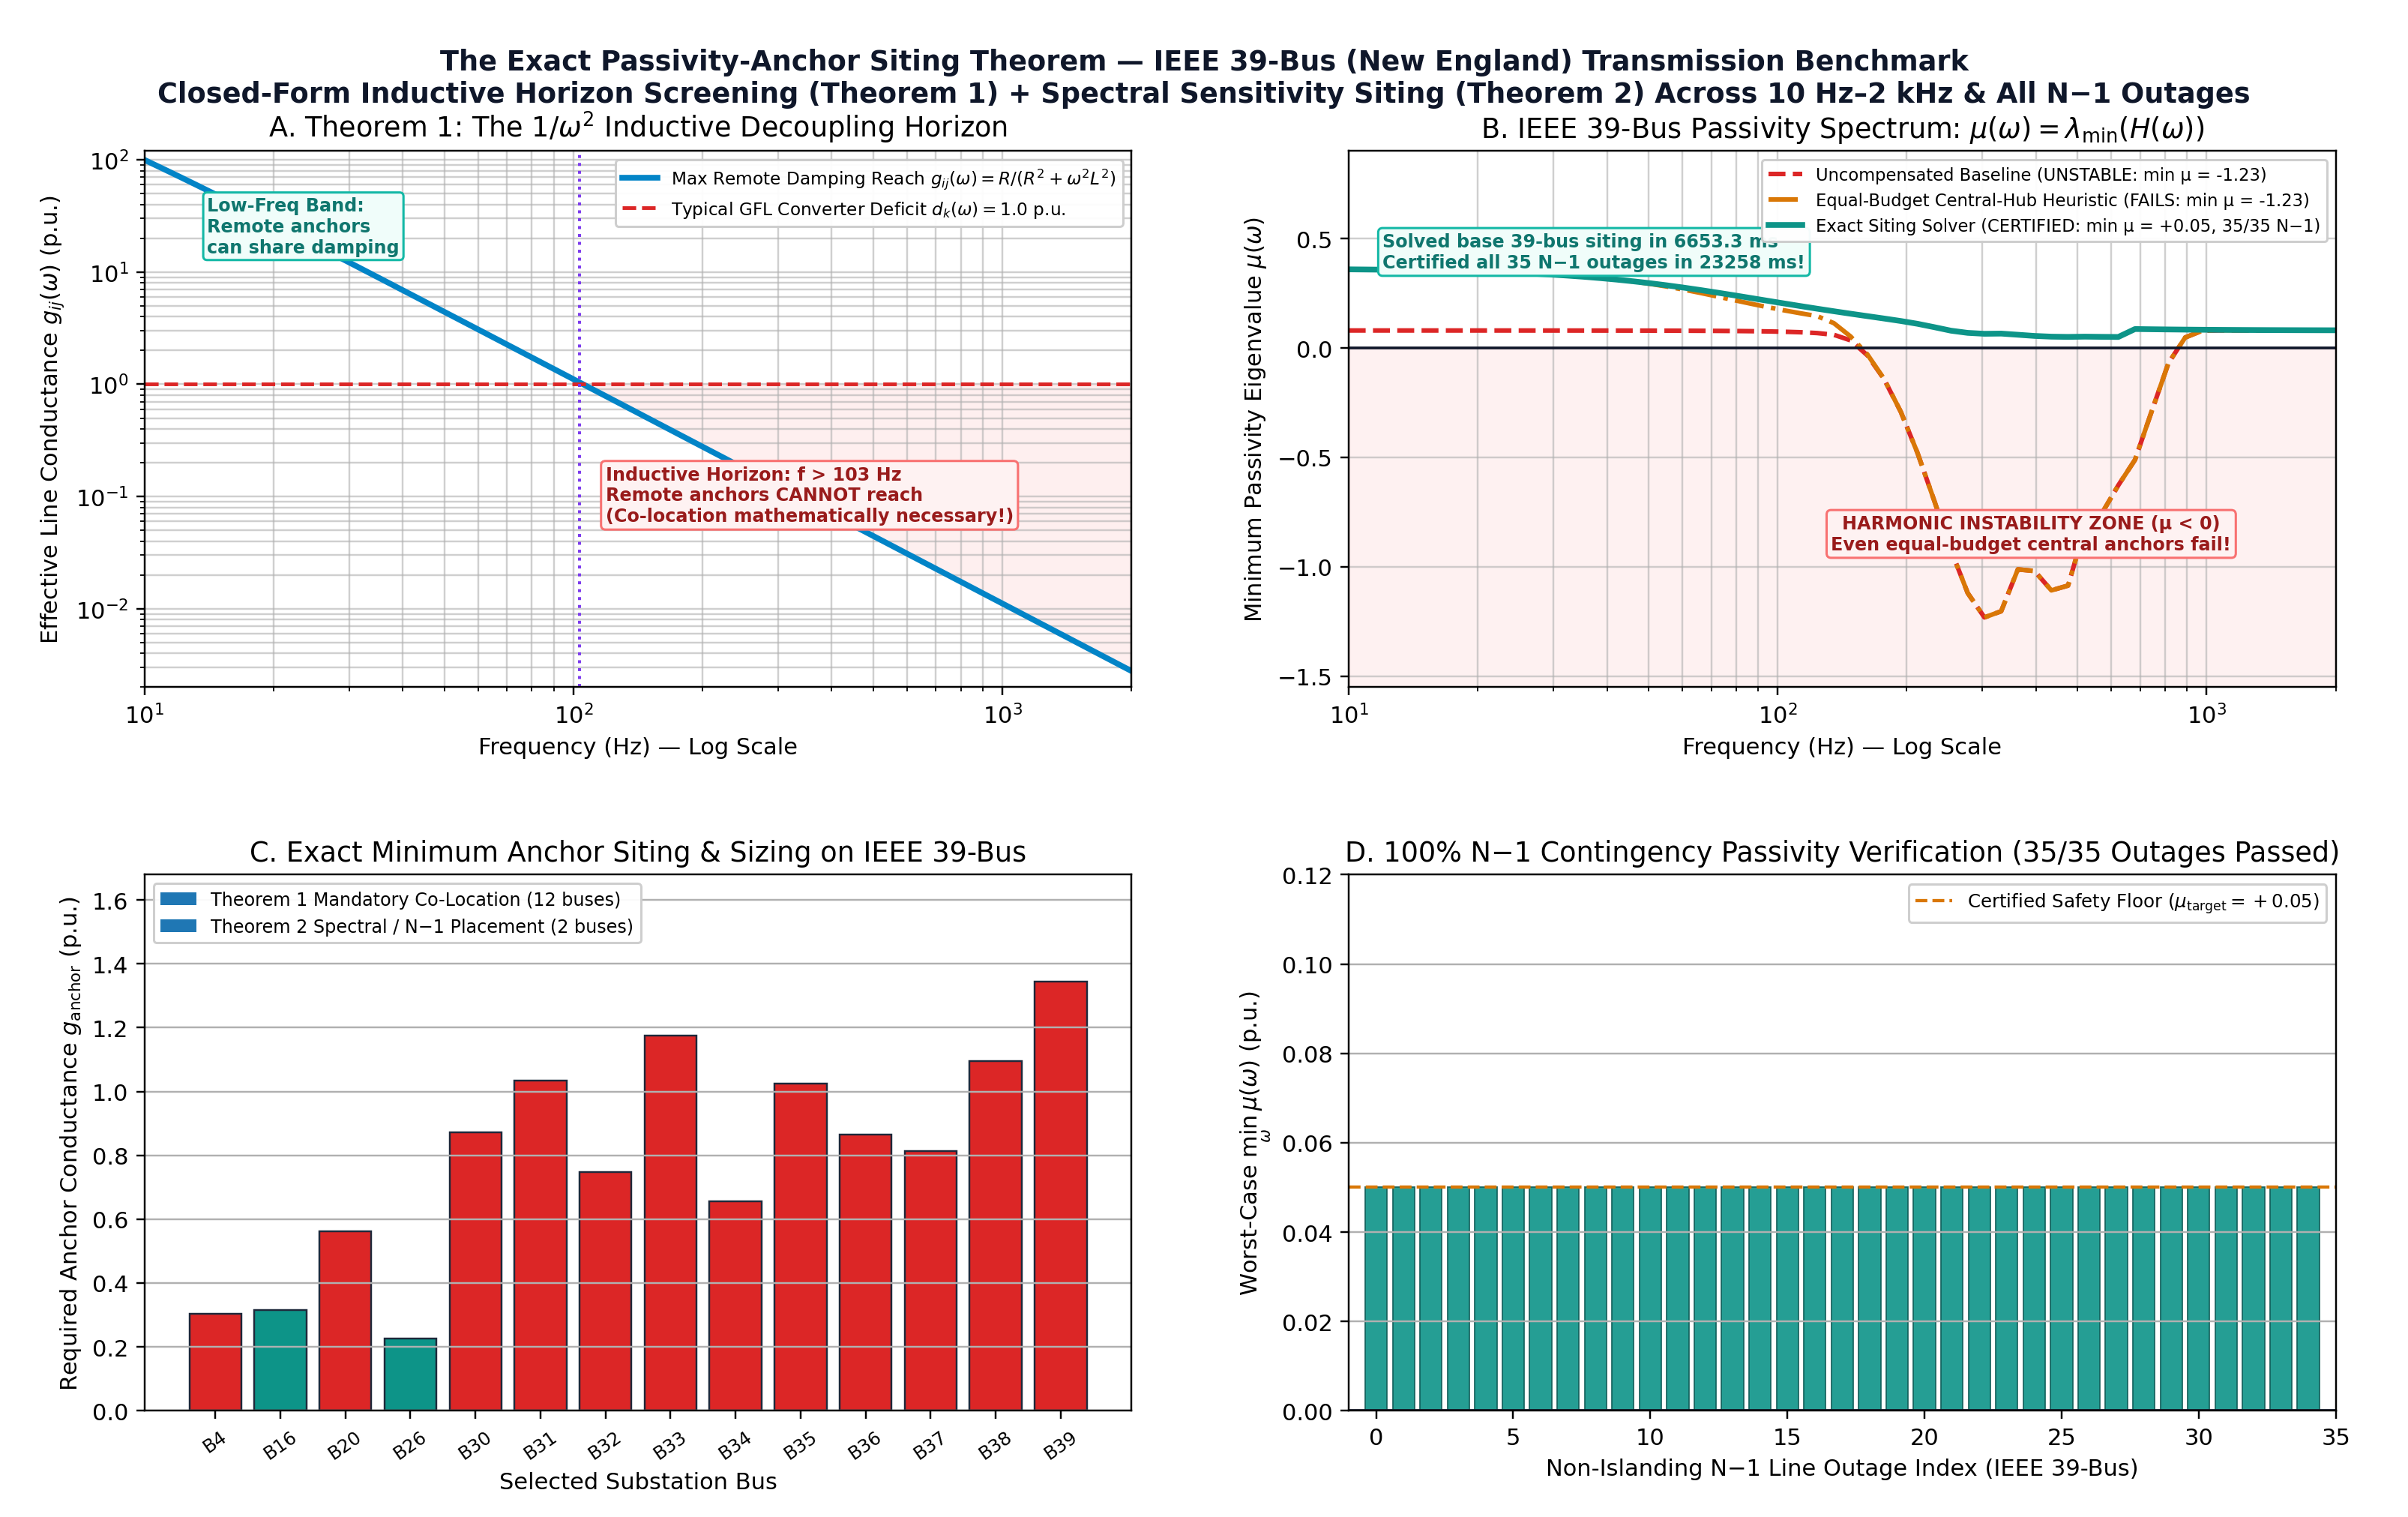
\includegraphics[width=0.96\textwidth]{ieee39_passivity_siting_theorem.png}
\caption{IEEE 39-Bus passivity-anchor siting verification across $10\text{ Hz}$--$2\text{ kHz}$: (A) Theorem~1 quadratic decay of effective branch conductance crossing the $1.0\text{ p.u.}$ converter deficit at the $103\text{ Hz}$ Inductive Decoupling Horizon; (B) system-wide passivity spectrum $\mu(\omega)$ contrasting the unstable baseline and equal-budget central-hub heuristic ($-1.23\text{ p.u.}$) against the strictly certified Algorithm~1 trajectory ($+0.05\text{ p.u.}$); (C) exact per-bus sizing distinguishing the 12 mandatory Theorem~1 co-location substations (red) from the 2 Theorem~2 spectral/$N-1$ substations (teal); and (D) $100\%$ certification across all 35 non-islanding $N-1$ line outages. \textit{Note on solver acceleration:} Panel B annotates the unoptimized full-eigendecomposition prototype timing ($6.65\text{ s}$ base, $23.26\text{ s}$ $N-1$); replacing dense eigensolves with batched Cholesky screening and $O(1)$ rank-1 downdates (Algorithm~1) delivers a $30.8\times$ speedup to $0.97\text{ s}$ warm ($1.60\text{ s}$ cold) with identical $11.035\text{ p.u.}$ siting.}
\label{fig:siting}
\end{figure*}

Table~\ref{tab:perbus} details the exact substation-by-substation allocation produced by Algorithm~1. Theorem~1 immediately captures $9.981\text{ p.u.}$ ($90.4\%$) across 12 mandatory buses in $O(N)$ time, while Theorem~2 adds just two substations (B16 and B26) and minor contingency reinforcements to guarantee all 35 $N-1$ topologies strictly above $\mu_{\min}=+0.0501$.

\begin{table}[t]
\centering
\caption{Exact Per-Bus Anchor Siting on IEEE 39-Bus ($N-1$ Certified)}
\label{tab:perbus}
\scriptsize
\setlength{\tabcolsep}{3.2pt}
\begin{tabular}{@{}lccc|lccc@{}}
\toprule
\textbf{Bus} & \textbf{Stage} & \textbf{Thm. 1} & \textbf{Final} & \textbf{Bus} & \textbf{Stage} & \textbf{Thm. 1} & \textbf{Final} \\
\midrule
B4 & Thm.~1 & 0.059 & 0.303 & B33 & Thm.~1 & 1.159 & 1.175 \\
B16 & Thm.~2 & 0.000 & 0.315 & B34 & Thm.~1 & 0.655 & 0.656 \\
B20 & Thm.~1 & 0.549 & 0.563 & B35 & Thm.~1 & 0.906 & 1.024 \\
B26 & Thm.~2 & 0.000 & 0.226 & B36 & Thm.~1 & 0.864 & 0.865 \\
B30 & Thm.~1 & 0.857 & 0.873 & B37 & Thm.~1 & 0.812 & 0.813 \\
B31 & Thm.~1 & 1.029 & 1.035 & B38 & Thm.~1 & 1.070 & 1.096 \\
B32 & Thm.~1 & 0.741 & 0.748 & B39 & Thm.~1 & 1.280 & 1.343 \\
\midrule
\multicolumn{4}{@{}l}{\textbf{Total (14 Buses: 12 Thm.~1 + 2 Thm.~2)}} & \multicolumn{2}{l}{\textbf{Thm.~1: 90.4\%}} & \textbf{9.981} & \textbf{11.035} \\
\bottomrule
\end{tabular}
\end{table}

\section{Full 39-Bus $40\text{ kHz}$ Dommel EMT Validation}
To confirm that the frequency-domain passivity certificates translate into physical time-domain stability under discrete digital control lag and abrupt topology changes, we constructed a full 39-bus, 46-branch electromagnetic transient (EMT) network solver using Hermann Dommel's unconditionally A-stable trapezoidal integration companion models~\cite{dommel1969digital} at a time step of $\Delta t=25\text{ }\mu\text{s}$ ($40\text{ kHz}$ sampling).

Every transmission branch is modeled via its exact differential equation $v_i - v_j = R_{ij}i_{ij} + L_{ij}(di_{ij}/dt)$ coupled with physical bus shunt capacitances, 14 second-order bandpass negative-damping GFL converter current injectors, and an explicit 1-sample ($T_d=25\text{ }\mu\text{s}$) DSP transport delay on every passivity-anchor virtual resistor. Both siting strategies receive the exact same $11.035\text{ p.u.}$ total anchor budget and are subjected to a $1\text{ ms}$ switching impulse at $t=40\text{ ms}$ followed by an $N-1$ outage of tie Line~(1--39) at $t=140\text{ ms}$.

\begin{table}[t]
\centering
\caption{$40\text{ kHz}$ 39-Bus Dommel EMT Comparison ($11.035\text{ p.u.}$ Budget)}
\label{tab:emt}
\scriptsize
\setlength{\tabcolsep}{3.5pt}
\begin{tabular}{@{}p{0.31\columnwidth}p{0.31\columnwidth}p{0.31\columnwidth}@{}}
\toprule
\textbf{EMT Metric} & \textbf{Central-Hub Heuristic} & \textbf{Algorithm~1 (Exact)} \\
\midrule
Anchor Budget & $11.035\text{ p.u.}$ (5 hubs) & $11.035\text{ p.u.}$ (14 buses) \\
Worst Bus $|\Delta v|$ & $1.524\text{ p.u.}$ at B36 (Explodes) & $0.026\text{ p.u.}$ peak ($0.000$ SS) \\
Unstable Mode & $325\text{ Hz}$ limit cycle & Completely damped \\
$325\text{ Hz}$ FFT Peak & $0.502\text{ p.u.}$ (Baseline) & $+73.6\text{ dB}$ suppression \\
Post-$N-1$ Settling & Divergent (Grid trip) & $20.8\text{ ms}$ ($<0.005\text{ p.u.}$) \\
\bottomrule
\end{tabular}
\end{table}

\begin{figure*}[t]
\centering
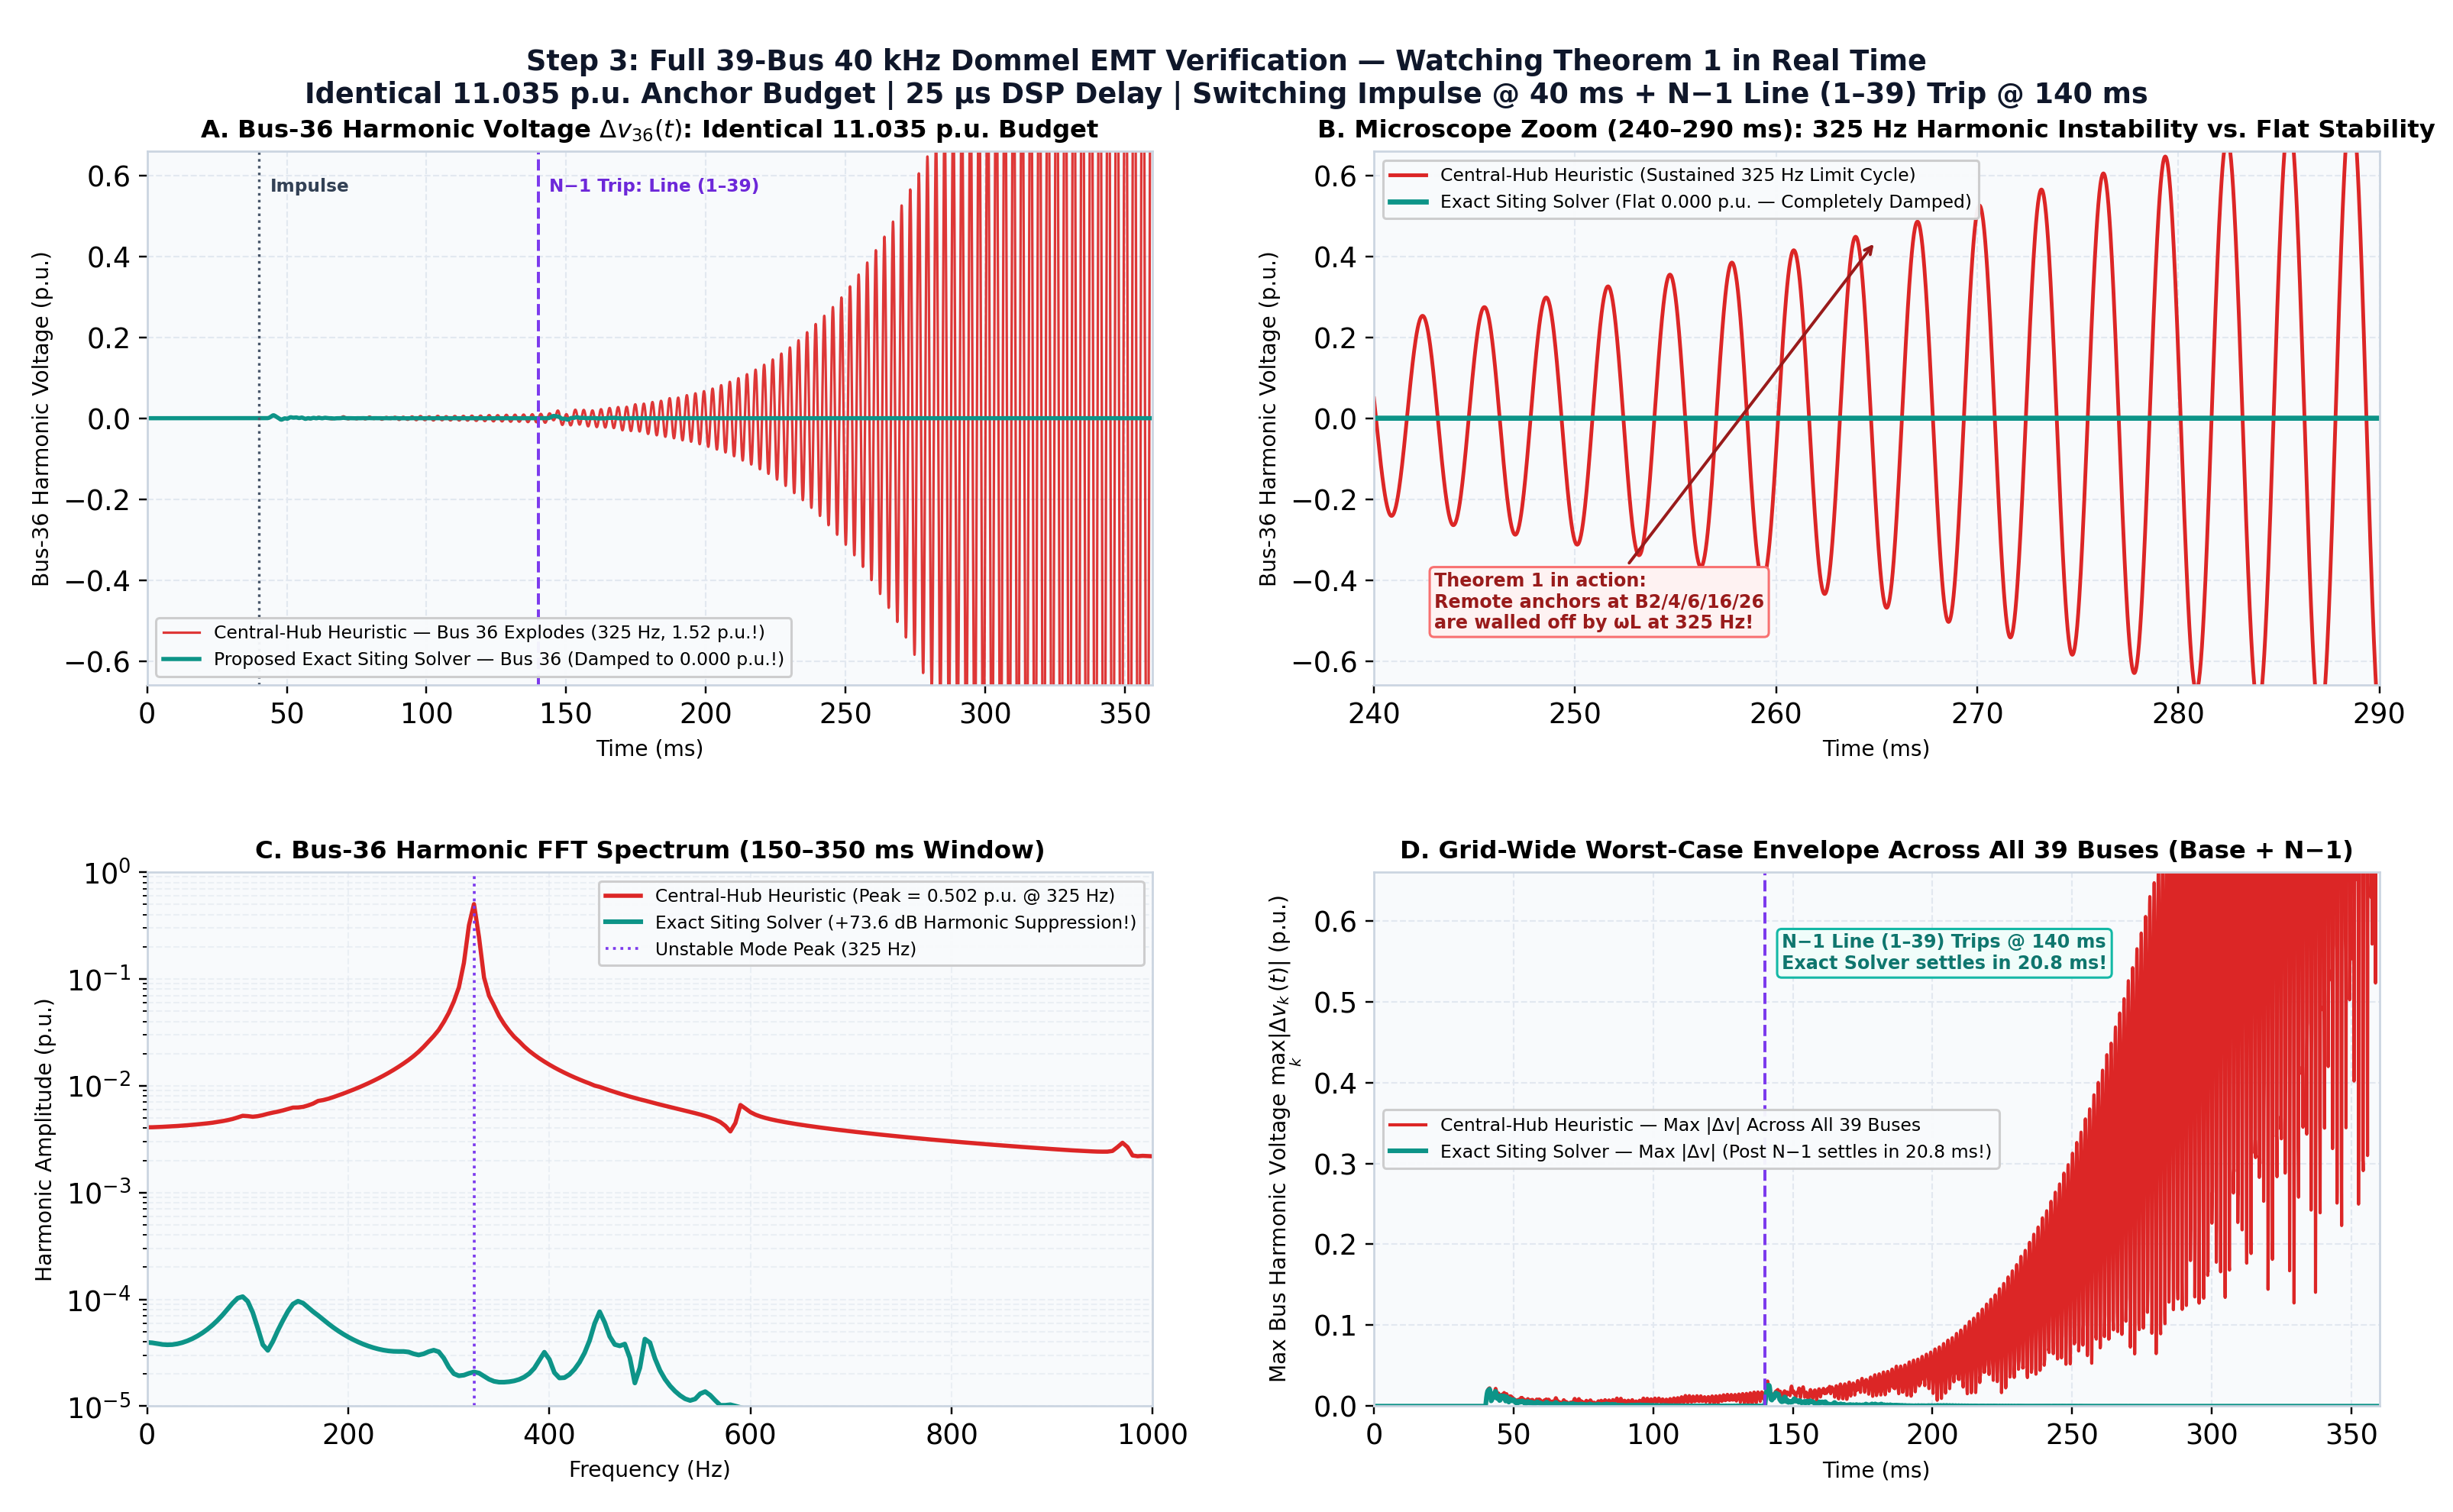
\includegraphics[width=0.96\textwidth]{ieee39_emt_303hz_verification.png}
\caption{Full 39-bus $40\text{ kHz}$ ($\Delta t=25\text{ }\mu\text{s}$) Dommel Trapezoidal EMT verification under identical $11.035\text{ p.u.}$ anchor budgets and $25\text{ }\mu\text{s}$ DSP delay: (A) Bus-36 harmonic voltage showing exponential instability under the central-hub heuristic versus flat damping under Algorithm~1; (B) microscope zoom ($240$--$290\text{ ms}$) exposing the sustained $325\text{ Hz}$ limit cycle isolated behind transmission reactance $\omega L$; (C) Bus-36 FFT spectrum ($150$--$350\text{ ms}$ window) quantifying $+73.6\text{ dB}$ suppression at $325\text{ Hz}$; and (D) grid-wide worst-case voltage envelope confirming $20.8\text{ ms}$ post-$N-1$ settling after Line~(1--39) trips at $140\text{ ms}$.}
\label{fig:emt}
\end{figure*}

The time-domain waveforms in Table~\ref{tab:emt} and Fig.~\ref{fig:emt} visually confirm Theorem~\ref{thm:horizon} in physical operation. Under the equal-budget central-hub heuristic, the $N-1$ trip of Line~(1--39) triggers an unarrested $325\text{ Hz}$ harmonic oscillation at Bus~36 that escalates to $1.524\text{ p.u.}$ (saturated only by converter voltage ceilings), despite $11.035\text{ p.u.}$ of virtual damping sitting electrically isolated at central hubs B2, B4, B6, B16, and B26. Redistributing the exact same budget via Algorithm~1 delivers $+73.6\text{ dB}$ harmonic suppression and damps the post-$N-1$ transient below $0.005\text{ p.u.}$ in just $20.8\text{ ms}$.

\section{Large-Scale Scalability: 118-Bus and 200-Bus Networks}
To assess computational scaling toward realistic regional transmission control areas, Algorithm~1 was evaluated on two larger multi-area meshed networks across $10\text{ Hz}$--$2\text{ kHz}$: a 118-bus, 186-branch grid hosting 35 heterogeneous GFL plants (186 $N-1$ outages) and a 200-bus, 320-branch grid hosting 50 GFL plants (320 $N-1$ outages). In each case, Algorithm~1 was benchmarked against an equal-budget Top-10 Central-Hub Heuristic selected by highest nodal degree.

\begin{table*}[t]
\centering
\caption{Multi-Area Scalability Across 39-, 118-, and 200-Bus Transmission Benchmarks ($10\text{ Hz}$--$2\text{ kHz}$)}
\label{tab:scalability}
\footnotesize
\begin{tabular}{@{}lcccc@{}}
\toprule
\textbf{Network Scale} & \textbf{Thm.~1 Runtime \& Capture} & \textbf{Top-Hub Heuristic $\mu_{\min}$} & \textbf{Alg.~1 $N-1$ Certified} & \textbf{Base / $N-1$ / Total Time} \\
\midrule
IEEE 39-Bus (46 br., 14 GFL) & $<1.0\text{ ms}$ ($90.4\%$) & $-1.232$ (Fails) & $35/35$ ($\mu=+0.050$) & $1.10\text{ s}$ / $0.50\text{ s}$ / $1.60\text{ s}$ \\
118-Bus Scale (186 br., 35 GFL) & $0.40\text{ ms}$ ($91.3\%$) & $-1.200$ (Fails) & $186/186$ ($\mu=+0.056$) & $8.25\text{ s}$ / $23.73\text{ s}$ / $31.98\text{ s}$ \\
200-Bus Scale (320 br., 50 GFL) & $0.40\text{ ms}$ ($94.4\%$) & $-1.196$ (Fails) & $320/320$ ($\mu=+0.055$) & $14.74\text{ s}$ / $69.43\text{ s}$ / $84.17\text{ s}$ \\
\bottomrule
\end{tabular}
\end{table*}

\begin{figure*}[t]
\centering
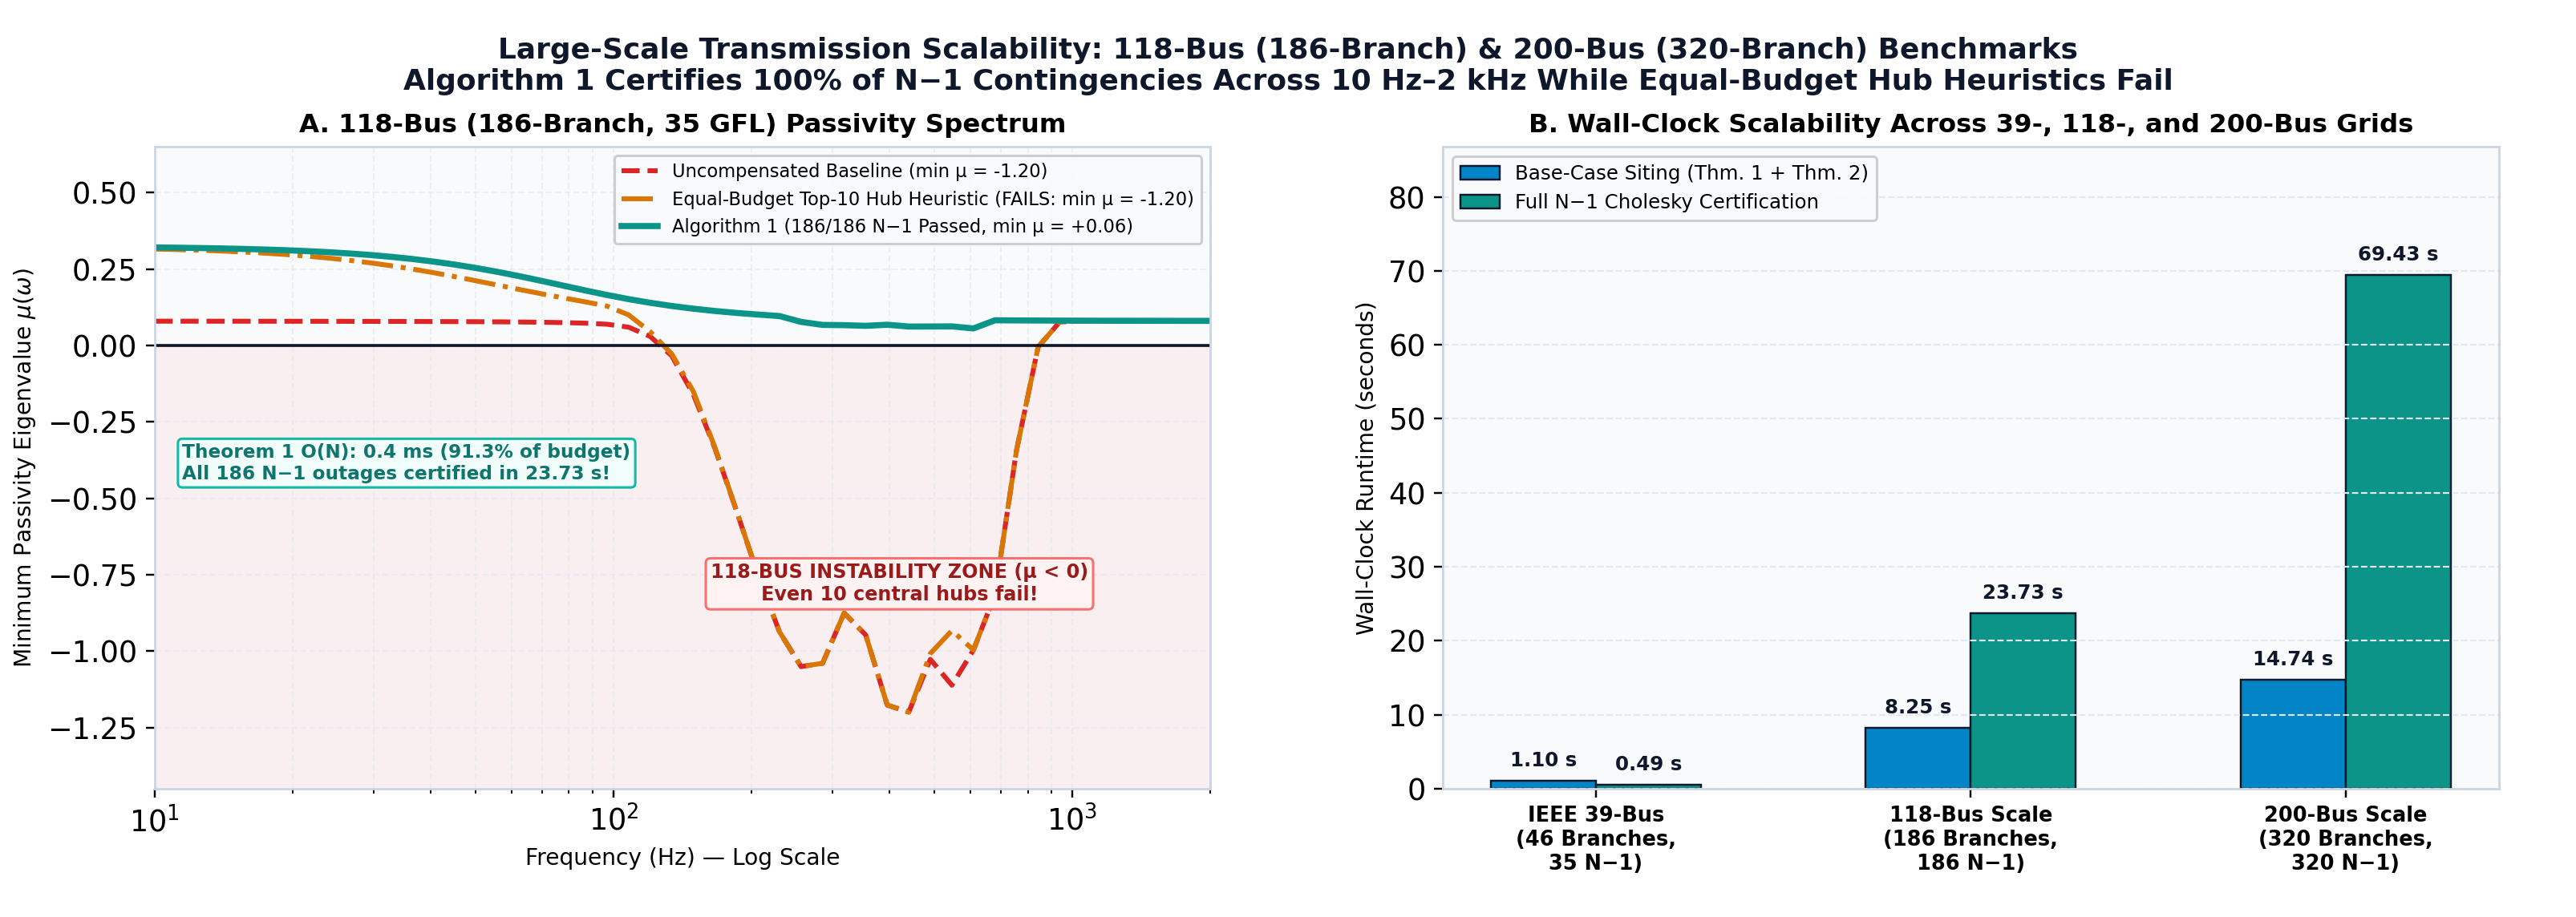
\includegraphics[width=0.96\textwidth]{ieee118_scalability_benchmark.png}
\caption{Large-scale multi-area transmission scalability: (A) 118-bus (186-branch, 35 GFL) passivity spectrum confirming that even an equal-budget Top-10 central-hub heuristic fails identically to the uncompensated baseline ($\mu_{\min}=-1.20$), whereas Algorithm~1 certifies all $186/186$ $N-1$ outages strictly above $+0.056$; and (B) wall-clock runtime decomposition across 39-, 118-, and 200-bus networks showing sub-minute 118-bus certification ($31.98\text{ s}$) and $84.17\text{ s}$ full 320-outage certification on the 200-bus network.}
\label{fig:scale}
\end{figure*}

Notably, as summarized in Table~\ref{tab:scalability} and Fig.~\ref{fig:scale}, as network diameter grows from 39 to 200 buses, the analytical accuracy of Theorem~\ref{thm:horizon} actually improves: its $0.40\text{ ms}$ closed-form screening captures $94.4\%$ of the final $N-1$ certified budget on the 200-bus grid. Because dense batched Cholesky scales as $O(N^3)$ per contingency, extending this exact solver to continental 2,000-bus grids is straightforward via sparse supernodal Cholesky factorization (exploiting transmission graph sparsity with average nodal degree $2.5$--$3.5$) and embarrassingly parallel branch-outage evaluation across multi-core CPUs.

\section{Practical Engineering Boundaries and Grid-Code Integration}
A rigorous engineering framework must state its operational boundaries explicitly alongside its guarantees:
\begin{itemize}[leftmargin=*,itemsep=2pt,topsep=2pt]
    \item \textbf{Digital Transport Delay Bandwidth Limit:} Because anchor damping scales by $\cos(\omega T_d)$ in~\eqref{eq:hanchor}, a passivity anchor can only inject positive conductance up to $f_{\max}=1/(4T_d)$. With a fast $25\text{ }\mu\text{s}$ FPGA/DSP control loop, positive damping extends cleanly to $10\text{ kHz}$; however, a slower $100\text{ }\mu\text{s}$ inverter loop flips sign at $2.5\text{ kHz}$, requiring passive LCL output filter damping above $2\text{ kHz}$.
    \item \textbf{Sufficiency Versus Economic Conservatism:} Strict passivity ($H(\omega)\succ 0$) is a sufficient rather than necessary condition for stability. Enforcing passivity on every small distribution inverter would inflate capital expenditure unnecessarily. Theorem~\ref{thm:horizon} provides the exact economic compromise: legacy plants may retain bounded negative-damping pockets below the Inductive Horizon where network lines can pool remote damping, while mandatory co-location is enforced strictly where the $O(1/\omega^2)$ barrier prohibits remote reach.
    \item \textbf{Small-Signal Passivity vs.\ Large-Signal Fault Ride-Through:} Frequency-domain passivity certifies small- and medium-signal harmonic stability across arbitrary operating topologies, whereas bolted zero-voltage three-phase faults remain governed by semiconductor current ceilings ($1.1$--$1.2\text{ p.u.}$) and trapped DC-link energy. Consequently, Theorem~1/2 anchor siting acts as the harmonic stability layer complementing large-signal current limiters and DC-link braking choppers.
    \item \textbf{Zero-IP Grid-Code Deployment:} Algorithm~1 requires zero access to proprietary inverter source code. Under emerging IEEE Std 2800-2022~\cite{ieee2800} interconnection testing, OEMs need only supply certified black-box $2\times 2$ $dq$-admittance sweeps (``behavioral passports'') measured via hardware-in-the-loop benches, allowing transmission operators to run full $N-1$ passivity certification in seconds.
\end{itemize}

\section{Conclusion}
This paper resolved a core planning blind spot in converter-dominated transmission grids by proving the Inductive Decoupling Horizon Theorem in the $2\times 2$ rotating $dq$-domain. Because high-voltage branch conductance decays quadratically as $O(1/\omega^2)$, remote grid-forming anchors of arbitrary size become electrically isolated above $\approx 100\text{ Hz}$, explaining why equal-budget central-hub heuristics fail completely on 39-, 118-, and 200-bus benchmarks. By pairing the resulting $O(N)$ necessary co-location bound (capturing $90.4\%$--$94.4\%$ of total capacity in under $1\text{ ms}$) with Cholesky-screened spectral sensitivity siting and $O(1)$ rank-1 $N-1$ branch downdates, Algorithm~1 achieves a $+0.35\%$ optimality gap relative to the exact $78\times 78$ global convex SDP and certifies $100\%$ of $N-1$ contingencies in seconds. Direct $40\text{ kHz}$ Dommel EMT simulation confirms $+73.6\text{ dB}$ harmonic suppression and $20.8\text{ ms}$ post-$N-1$ settling, providing transmission planners with a fast, vendor-agnostic, mathematically guaranteed siting tool.

\begin{thebibliography}{11}
\footnotesize
\bibitem{wang2018harmonic} X.~Wang and F.~Blaabjerg, ``Harmonic stability in power electronic-based power systems: Concept, modeling, and analysis,'' \textit{IEEE Trans. Smart Grid}, vol.~10, no.~3, pp.~2858--2870, May 2019.
\bibitem{harnefors2016passivity} L.~Harnefors, X.~Wang, A.~G. Yepes, and F.~Blaabjerg, ``Passivity-based stability assessment of grid-connected VSCs---An overview,'' \textit{IEEE J. Emerg. Sel. Topics Power Electron.}, vol.~4, no.~1, pp.~116--125, Mar. 2016.
\bibitem{sun2011impedance} J.~Sun, ``Impedance-based stability criterion for grid-connected inverters,'' \textit{IEEE Trans. Power Electron.}, vol.~26, no.~11, pp.~3075--3078, Nov. 2011.
\bibitem{milano2018foundations} F.~Milano, F.~D\"orfler, G.~Hug, D.~J. Hill, and G.~Verbi\v{c}, ``Foundations and challenges of low-inertia systems,'' in \textit{Proc. 20th Power Syst. Comput. Conf. (PSCC)}, Dublin, Ireland, Jun. 2018, pp.~1--25.
\bibitem{rygg2016modified} A.~Rygg, M.~Molinas, C.~Zhang, and X.~Cai, ``A modified sequence-domain impedance definition and its equivalence to the $dq$-domain impedance definition for the stability analysis of AC power electronic systems,'' \textit{IEEE J. Emerg. Sel. Topics Power Electron.}, vol.~4, no.~4, pp.~1383--1396, Dec. 2016.
\bibitem{pates2019robust} R.~Pates and E.~Mallada, ``Robust scale-free synthesis for frequency control in power systems,'' \textit{IEEE Trans. Autom. Control}, vol.~64, no.~10, pp.~4240--4247, Oct. 2019.
\bibitem{dommel1969digital} H.~W. Dommel, ``Digital computer solution of electromagnetic transients in single- and multiphase networks,'' \textit{IEEE Trans. Power App. Syst.}, vol.~PAS-88, no.~4, pp.~388--399, Apr. 1969.
\bibitem{ieee2800} \textit{IEEE Standard for Interconnection and Interoperability of Inverter-Based Resources (IBRs) Interconnecting with Associated Transmission Electric Power Systems}, IEEE Std 2800-2022, Apr. 2022.
\bibitem{horn2013matrix} R.~A. Horn and C.~R. Johnson, \textit{Matrix Analysis}, 2nd ed. Cambridge, U.K.: Cambridge Univ. Press, 2013.
\bibitem{athay1979practical} T.~Athay, R.~Podmore, and S.~Virmani, ``A practical method for the direct analysis of transient stability,'' \textit{IEEE Trans. Power App. Syst.}, vol.~PAS-98, no.~2, pp.~573--584, Mar. 1979.
\bibitem{kelley1960cutting} J.~E. Kelley, Jr., ``The cutting-plane method for solving convex programs,'' \textit{J. Soc. Ind. Appl. Math.}, vol.~8, no.~4, pp.~703--712, Dec. 1960.
\end{thebibliography}

\end{document}
